\documentclass[11pt,a4paper]{report}
\usepackage[utf8]{inputenc}
\usepackage{geometry}
\geometry{margin=1in}
\usepackage{graphicx}
\usepackage{setspace}
\usepackage{titlesec}
\usepackage{longtable}
\usepackage{booktabs}
\usepackage{array}
\usepackage{amsmath}
\usepackage{listings}
\usepackage{xcolor}
\usepackage{hyperref}

\hypersetup{
    colorlinks=true,
    linkcolor=black,
    urlcolor=blue,
    citecolor=black
}

\setcounter{secnumdepth}{3}
\renewcommand{\thesection}{\arabic{section}}

% Code snippet styling
\lstset{
    basicstyle=\ttfamily\footnotesize,
    breaklines=true,
    frame=single,
    backgroundcolor=\color{gray!10},
    numbers=none,
    showstringspaces=false
}

\begin{document}

% ------------------ Title Page ------------------
\begin{titlepage}
    \centering
   
    
\includegraphics[width=3.4cm,height=2.6cm]{College Logo Grayscale.jpg}\\[0.5cm]

    \vspace{0.8cm}
    \textbf{\large A Course End Project Report on} \\[0.5cm]
    {\LARGE \textbf{ATM Transaction System}}\\[1.2cm]
    {\Large A9510 - Database Management System Laboratory}\\[1.2cm]
    \textbf{Submitted by}\\ [0.25cm]
    Batch No. 2026-DBMS-B1 

\begin{center}
	\begin{table}[h!]
		\centering
        \setstretch{1.1}
		\begin{tabular}{l l}
			{Student Name 1} & {Roll No - 1}\\ [2mm]
			{Student Name 2} & {Roll No - 2}\\ [2mm]
			{Student Name 3} & {Roll No - 3}\\ [2mm]
		\end{tabular} 
	\end{table}
\end{center}
    \vspace{0.5cm}
    \textbf{Course Facilitator}\\ [0.075in]
    Mr. Prasada Reddy G S\\
    Assistant Professor, Department of CSE\\[1.8cm]

    {\large\textbf{Department of Computer Science and Engineering}}\\[0.4cm]
    {\large\textbf{Vardhaman College of Engineering, Hyderabad}}\\[0.4cm]
    {\large \textbf{Academic Year 2026--2027}}
\end{titlepage}

% ------------------ Preliminary Pages ------------------
\tableofcontents
\newpage

\section*{Abstract}
\addcontentsline{toc}{section}{Abstract}
\noindent Traditional banking branch operations for routine monetary tasks—such as balance inquiries, cash withdrawals, cash deposits, and peer-to-peer account transfers—suffer from physical delays, high operational overhead, manual record discrepancies, and vulnerability to concurrency anomalies. An Automated Teller Machine (ATM) transaction system serves as a foundational paradigm of modern distributed financial technology, demonstrating critical database management concepts including strict atomicity, consistency, isolation, and durability (ACID), normalized relational schema modeling, data security, and concurrent transaction control.

This project presents the design, architectural modeling, database implementation, and desktop application of a complete, educational \textbf{ATM Transaction System}. Built upon an enterprise-grade relational database schema comprising seven normalized tables (\texttt{customers}, \texttt{accounts}, \texttt{atm\_cards}, \texttt{transactions}, \texttt{transfers}, \texttt{admins}, and \texttt{login\_attempts}) engineered in MySQL 8.x (InnoDB engine), the system guarantees strict integrity through primary keys, foreign key constraints with cascade updates, CHECK constraints preventing negative balances, and unique candidate keys. Data normalization is rigorously analyzed and demonstrated up to Boyce-Codd Normal Form (BCNF). Application logic is implemented in Java 21 adhering to a clean 3-Tier Layered Architecture (Presentation, Service, Data Access via JDBC Connection Pooling). Cryptographic protection enforces one-way BCrypt hashing (cost factor 12) for customer PINs and administrative credentials, completely eliminating plaintext password storage. Concurrency control and race-condition prevention are achieved through atomic conditional database updates (\texttt{UPDATE accounts SET balance = balance - :amount WHERE account\_id = :id AND balance >= :amount}) and isolated transactional boundaries. 

The user interface delivers a high-fidelity desktop experience inspired by modern dark fintech design paradigms (Sight Banking and Contiant), incorporating emerald green and cyan visual tokens, responsive card layouts, and complete user session isolation. A comprehensive 45-case automated test suite was developed and executed, validating functional workflows, transaction rollbacks, denomination limits, brute-force lockout safeguards, and multi-threaded race conditions with a 100\% pass rate.

\vspace{0.5cm}
\noindent \textbf{Keywords}: Database Management System, ATM Transaction System, Relational Schema, ACID Properties, Normalization (3NF/BCNF), BCrypt Hashing, Concurrency Control, Java Swing, JDBC Connection Pool.

\newpage

% ------------------ Chapter 1: Introduction ------------------
\section{Introduction}

\subsection{Background of the Problem}
Financial institutions process millions of electronic transactions daily. Before the widespread deployment of Automated Teller Machines, customers were compelled to visit brick-and-mortar bank branches during limited operational hours to execute routine tasks such as withdrawing funds, depositing physical currency, transferring amounts, or inspecting account ledgers. Manual ledger keeping and legacy paper workflows introduced severe bottlenecks, human accounting errors, ledger reconciliation delays, and risks of double spending or unrecorded disbursements.

The Automated Teller Machine revolutionized retail banking by decentralizing access to core ledger operations. However, automating financial operations introduces profound software engineering and database integrity challenges. Because multiple terminals, cards, and online channels access central account balances simultaneously, financial databases must guarantee that no account balance is ever overdrawn, that transaction history records are never lost or corrupted, that system failures during execution never leave money in limbo, and that unauthorized parties cannot compromise sensitive credentials. A relational database management system (RDBMS) providing full transactional support is the essential foundation for solving these challenges.

\subsection{Problem Statement}
To design, model, implement, and verify a robust, normalized relational database and an accompanying Java desktop application for an educational \textbf{ATM Transaction System} that:
\begin{enumerate}
    \item Maintains structured records of customers, bank accounts, ATM cards, transactions, fund transfers, administrative personnel, and authentication audit logs.
    \item Enforces strict entity integrity, referential integrity, and domain constraints preventing negative account balances and invalid financial states.
    \item Implements ACID-compliant transactional workflows for cash withdrawals, cash deposits, and inter-account fund transfers, guaranteeing total rollback in case of partial failures.
    \item Provides secure credential verification utilizing salted, slow one-way cryptographic hashing (BCrypt) without storing plaintext PINs or passwords.
    \item Delivers a modern, intuitive graphical interface featuring separate ATM customer and administrative workflows.
\end{enumerate}

\subsection{Scope of the Project}
The scope of this project encompasses:
\begin{itemize}
    \item \textbf{Relational Database Schema}: Design of seven relational tables in MySQL 8.x with InnoDB storage engine, achieving Boyce-Codd Normal Form (BCNF).
    \item \textbf{Data Security}: Implementation of BCrypt PIN hashing (cost factor 12), protection against card enumeration attacks, and automated brute-force lockout after three consecutive failed authentication attempts.
    \item \textbf{Transaction Processing}: Atomic cash withdrawal, simulated deposit, and two-sided inter-account transfer utilizing JDBC transactions with explicit \texttt{commit()} and \texttt{rollback()} controls.
    \item \textbf{Desktop User Interface}: A Java Swing desktop interface adhering to modern fintech aesthetic principles (Sight Banking and Contiant), with masked credential inputs and real-time ledger updates.
    \item \textbf{Administrative Subsystem}: Dedicated administrative portal allowing authorized personnel to inspect ledger overviews, review audit trails, and manage card statuses (activation/blocking).
    \item \textbf{Automated Testing}: A suite of 45 automated unit and simulation test cases validating every system constraint and concurrency boundary.
\end{itemize}

\subsection{Objectives of the Project}
The primary technical and academic objectives of this project are:
\begin{itemize}
    \item To model and construct an entity-relationship diagram and normalized relational schema reflecting real-world banking relationships.
    \item To prove mathematical normalization up to BCNF, eliminating insertion, deletion, and update anomalies.
    \item To implement ACID transactional guarantees and explain their mechanisms in terms of atomicity, consistency, isolation, and durability.
    \item To demonstrate concurrency safety using atomic conditional SQL updates, preventing race-condition overdrafts during simultaneous withdrawals.
    \item To develop a clean 3-Tier Layered Architecture separating presentation (Swing), domain logic (Services), and database interactions (DAOs with JDBC connection pooling).
    \item To evaluate performance and map project achievements to ABET Program Outcomes and United Nations Sustainable Development Goals (SDGs).
\end{itemize}

\newpage

% ------------------ Chapter 2: Literature Review ------------------
\section{Literature Review}

\subsection{Existing Systems}
Retail banking and financial access systems have evolved through several historical paradigms:
\begin{enumerate}
    \item \textbf{Manual Ledger Branch Banking}: All account balances and entries were recorded in physical paper ledgers. Withdrawals required bank tellers to manually cross-reference signatures, inspect ledger sheets, and hand over cash. This system suffered from severe processing delays, geographic constraints, high staffing costs, and vulnerability to bookkeeping discrepancies.
    \item \textbf{Centralized Mainframe Batch Processing}: In early computational banking (1960s--1980s), transactions were collected throughout the business day on punch cards or magnetic tapes and processed in batch jobs overnight. While this reduced branch bookkeeping, account balances were only updated at the end of the day, allowing customers to overdraw funds by making withdrawals at multiple locations before batch reconciliation.
    \item \textbf{Online Distributed ATM Networks}: Contemporary ATMs connect over secure financial networks (e.g., Cirrus, Plus, National Financial Switch) to centralized core banking database engines. Transactions are executed in real time against relational or distributed databases using strict two-phase commit protocols and hardware security modules (HSMs).
\end{enumerate}

\subsection{Limitations of Existing Educational Implementations}
Many educational or introductory student projects simulating ATM systems suffer from critical architectural and database shortcomings:
\begin{itemize}
    \item \textbf{In-Memory Storage}: Storing accounts and card balances in memory data structures (e.g., Java \texttt{HashMap} or \texttt{ArrayList}) rather than a relational database, causing total data loss upon application termination.
    \item \textbf{Plaintext PIN Storage}: Storing user PINs and administrator passwords as raw plaintext strings or trivial invertible transformations, violating basic data privacy standards.
    \item \textbf{Absence of Transaction Isolation}: Performing balance debits and transaction logging as independent, non-transactional SQL queries, leaving the ledger corrupted if an error occurs midway.
    \item \textbf{Floating-Point Financial Data Types}: Using \texttt{float} or \texttt{double} types for monetary values, causing catastrophic rounding and precision errors over repeated calculations.
    \item \textbf{Vulnerability to SQL Injection}: Constructing dynamic SQL queries via string concatenation rather than parameterized prepared statements.
\end{itemize}

\subsection{Proposed Database System}
The system proposed in this report addresses every limitation identified above:
\begin{itemize}
    \item Complete persistence in MySQL InnoDB with referential constraints and automatic crash recovery.
    \item Use of exact \texttt{DECIMAL(15,2)} data types for all balances and amounts.
    \item Military-grade BCrypt hashing with unique random salts for every cardholder.
    \item Explicit JDBC transaction boundaries with atomic rollback on any failure.
    \item Fully parameterized \texttt{PreparedStatement} operations across all Data Access Objects.
    \item Atomic conditional updates eliminating race-condition overdrafts.
\end{itemize}

\newpage

% ------------------ Chapter 3: Problem Analysis ------------------
\section{Problem Analysis}

\subsection{Real-World Problem Description}
An ATM transaction terminal is a shared public kiosk interacting directly with customer bank accounts. When a customer inserts an ATM card and enters a Personal Identification Number (PIN), the terminal must authenticate the identity securely, query the current balance, validate that the requested withdrawal or transfer amount conforms to available funds and daily limits, dispense cash, update the account balance, and produce an immutable transaction log.

If two cardholders linked to a joint account simultaneously initiate withdrawals at separate terminals, the system must guarantee that both transactions do not simultaneously read the original balance and both dispense cash, which would cause an overdraft. Furthermore, if power fails or the network disconnects after the account is debited but before the transaction is logged, the entire operation must automatically roll back to restore the original account state.

\subsection{Users and Stakeholders}
The system identifies three primary categories of stakeholders:
\begin{enumerate}
    \item \textbf{ATM Cardholders / Customers}: End users seeking rapid, secure self-service banking operations including balance inquiry, cash withdrawal, cash deposit, fund transfer to peer accounts, and mini statement generation.
    \item \textbf{Bank Administrators}: Authorized operational personnel who monitor system health, inspect aggregated customer and account summaries, review audit trails, and unlock cards locked by brute-force triggers.
    \item \textbf{Database Architects and Auditors}: Stakeholders responsible for ensuring that financial ledgers comply with double-entry accounting standards, auditability, and regulatory security frameworks.
\end{enumerate}

\subsection{System Assumptions}
\begin{itemize}
    \item All monetary operations are denominated in Indian Rupees (INR, \symbol{150}) with a minimum unit of 1 paisa (0.01).
    \item Cash withdrawals and deposits must occur in multiples of ₹100, reflecting physical automated cash dispenser cassette capabilities.
    \item A cardholder's account balance cannot drop below the configured minimum balance (₹1,000.00 for Savings, ₹5,000.00 for Current).
    \item Maximum single-transaction withdrawal is configured to ₹25,000.00, and maximum daily cumulative withdrawal is configured to ₹100,000.00.
    \item Maximum consecutive failed PIN attempts is set to 3, triggering an automated 30-minute security lock.
\end{itemize}

\subsection{Functional Requirements}
\begin{itemize}
    \item \textbf{FR-1: Authentication}: Verification of card number and PIN using BCrypt. Lockout after 3 failed attempts.
    \item \textbf{FR-2: Balance Inquiry}: Real-time database query of available balance with zero in-memory caching.
    \item \textbf{FR-3: Cash Withdrawal}: Validation of positive amount, denomination (multiple of 100), per-transaction limit, daily limit, and balance sufficiency. Atomic debit and transaction insert.
    \item \textbf{FR-4: Cash Deposit}: Validation of positive amount and denomination. Atomic credit and transaction insert.
    \item \textbf{FR-5: Fund Transfer}: Validation of destination account existence, rejection of self-transfers, atomic debit of source and credit of destination linked by shared UUID reference.
    \item \textbf{FR-6: Mini Statement}: Retrieval of the 10 most recent transactions for the authenticated account, ordered newest first.
    \item \textbf{FR-7: Administrative Dashboard}: Segregated login, customer list, account overview, card activation/blocking, and system-wide transaction log inspection.
    \item \textbf{FR-8: Customer Sign-Up \& Card Issuance}: Dedicated registration interface allowing new users to open bank accounts, specify custom or auto-generated 16-digit card numbers (e.g., 4532-1234-5678-9010), establish BCrypt-hashed 4-digit PINs, and make opening deposits atomically.
\end{itemize}

\subsection{Non-Functional Requirements}
\begin{itemize}
    \item \textbf{Data Integrity}: Strict referential integrity; foreign key constraints; non-negative balance checks.
    \item \textbf{Security}: Zero plaintext PIN or password storage; prepared statements preventing SQL injection; generic authentication error messages preventing account enumeration.
    \item \textbf{Performance}: Sub-second query execution utilizing indexed primary and foreign keys; connection reuse via thread-safe JDBC connection pooling.
    \item \textbf{Reliability and ACID Compliance}: Complete transactional rollback on any runtime or database exception.
\end{itemize}

\newpage

% ------------------ Chapter 4: System Design ------------------
\section{System Design}

\subsection{Entity Relationship (ER) Model}
The ATM Transaction System is modeled around core entities representing retail banking operations:
\begin{itemize}
    \item \textbf{Customer}: Represents an individual bank customer, uniquely identified by \texttt{customer\_id}, holding attributes such as name, date of birth, contact details, and address.
    \item \textbf{Account}: Represents a financial ledger account linked to a customer, uniquely identified by \texttt{account\_id} and candidate key \texttt{account\_number}. Holds monetary attributes (\texttt{balance}, \texttt{min\_balance}) and status.
    \item \textbf{ATMCard}: Represents a physical credential tied to an account, identified by \texttt{card\_id} and unique \texttt{card\_number}. Stores cryptographic hash \texttt{pin\_hash}, status, and lockout metadata.
    \item \textbf{Transaction}: Represents an immutable monetary event, identified by \texttt{transaction\_id} and unique UUID \texttt{transaction\_ref}. Stores type, amount, resulting balance, timestamp, and foreign keys.
    \item \textbf{Transfer}: Represents an atomic transfer connecting a source account and a destination account with a shared reference.
    \item \textbf{Admin}: Represents an authorized bank administrator with credential hashes and system role.
    \item \textbf{LoginAttempt}: Represents an audit event recording all authentication requests for fraud monitoring.
\end{itemize}

\begin{figure}[htbp]
    \centering
    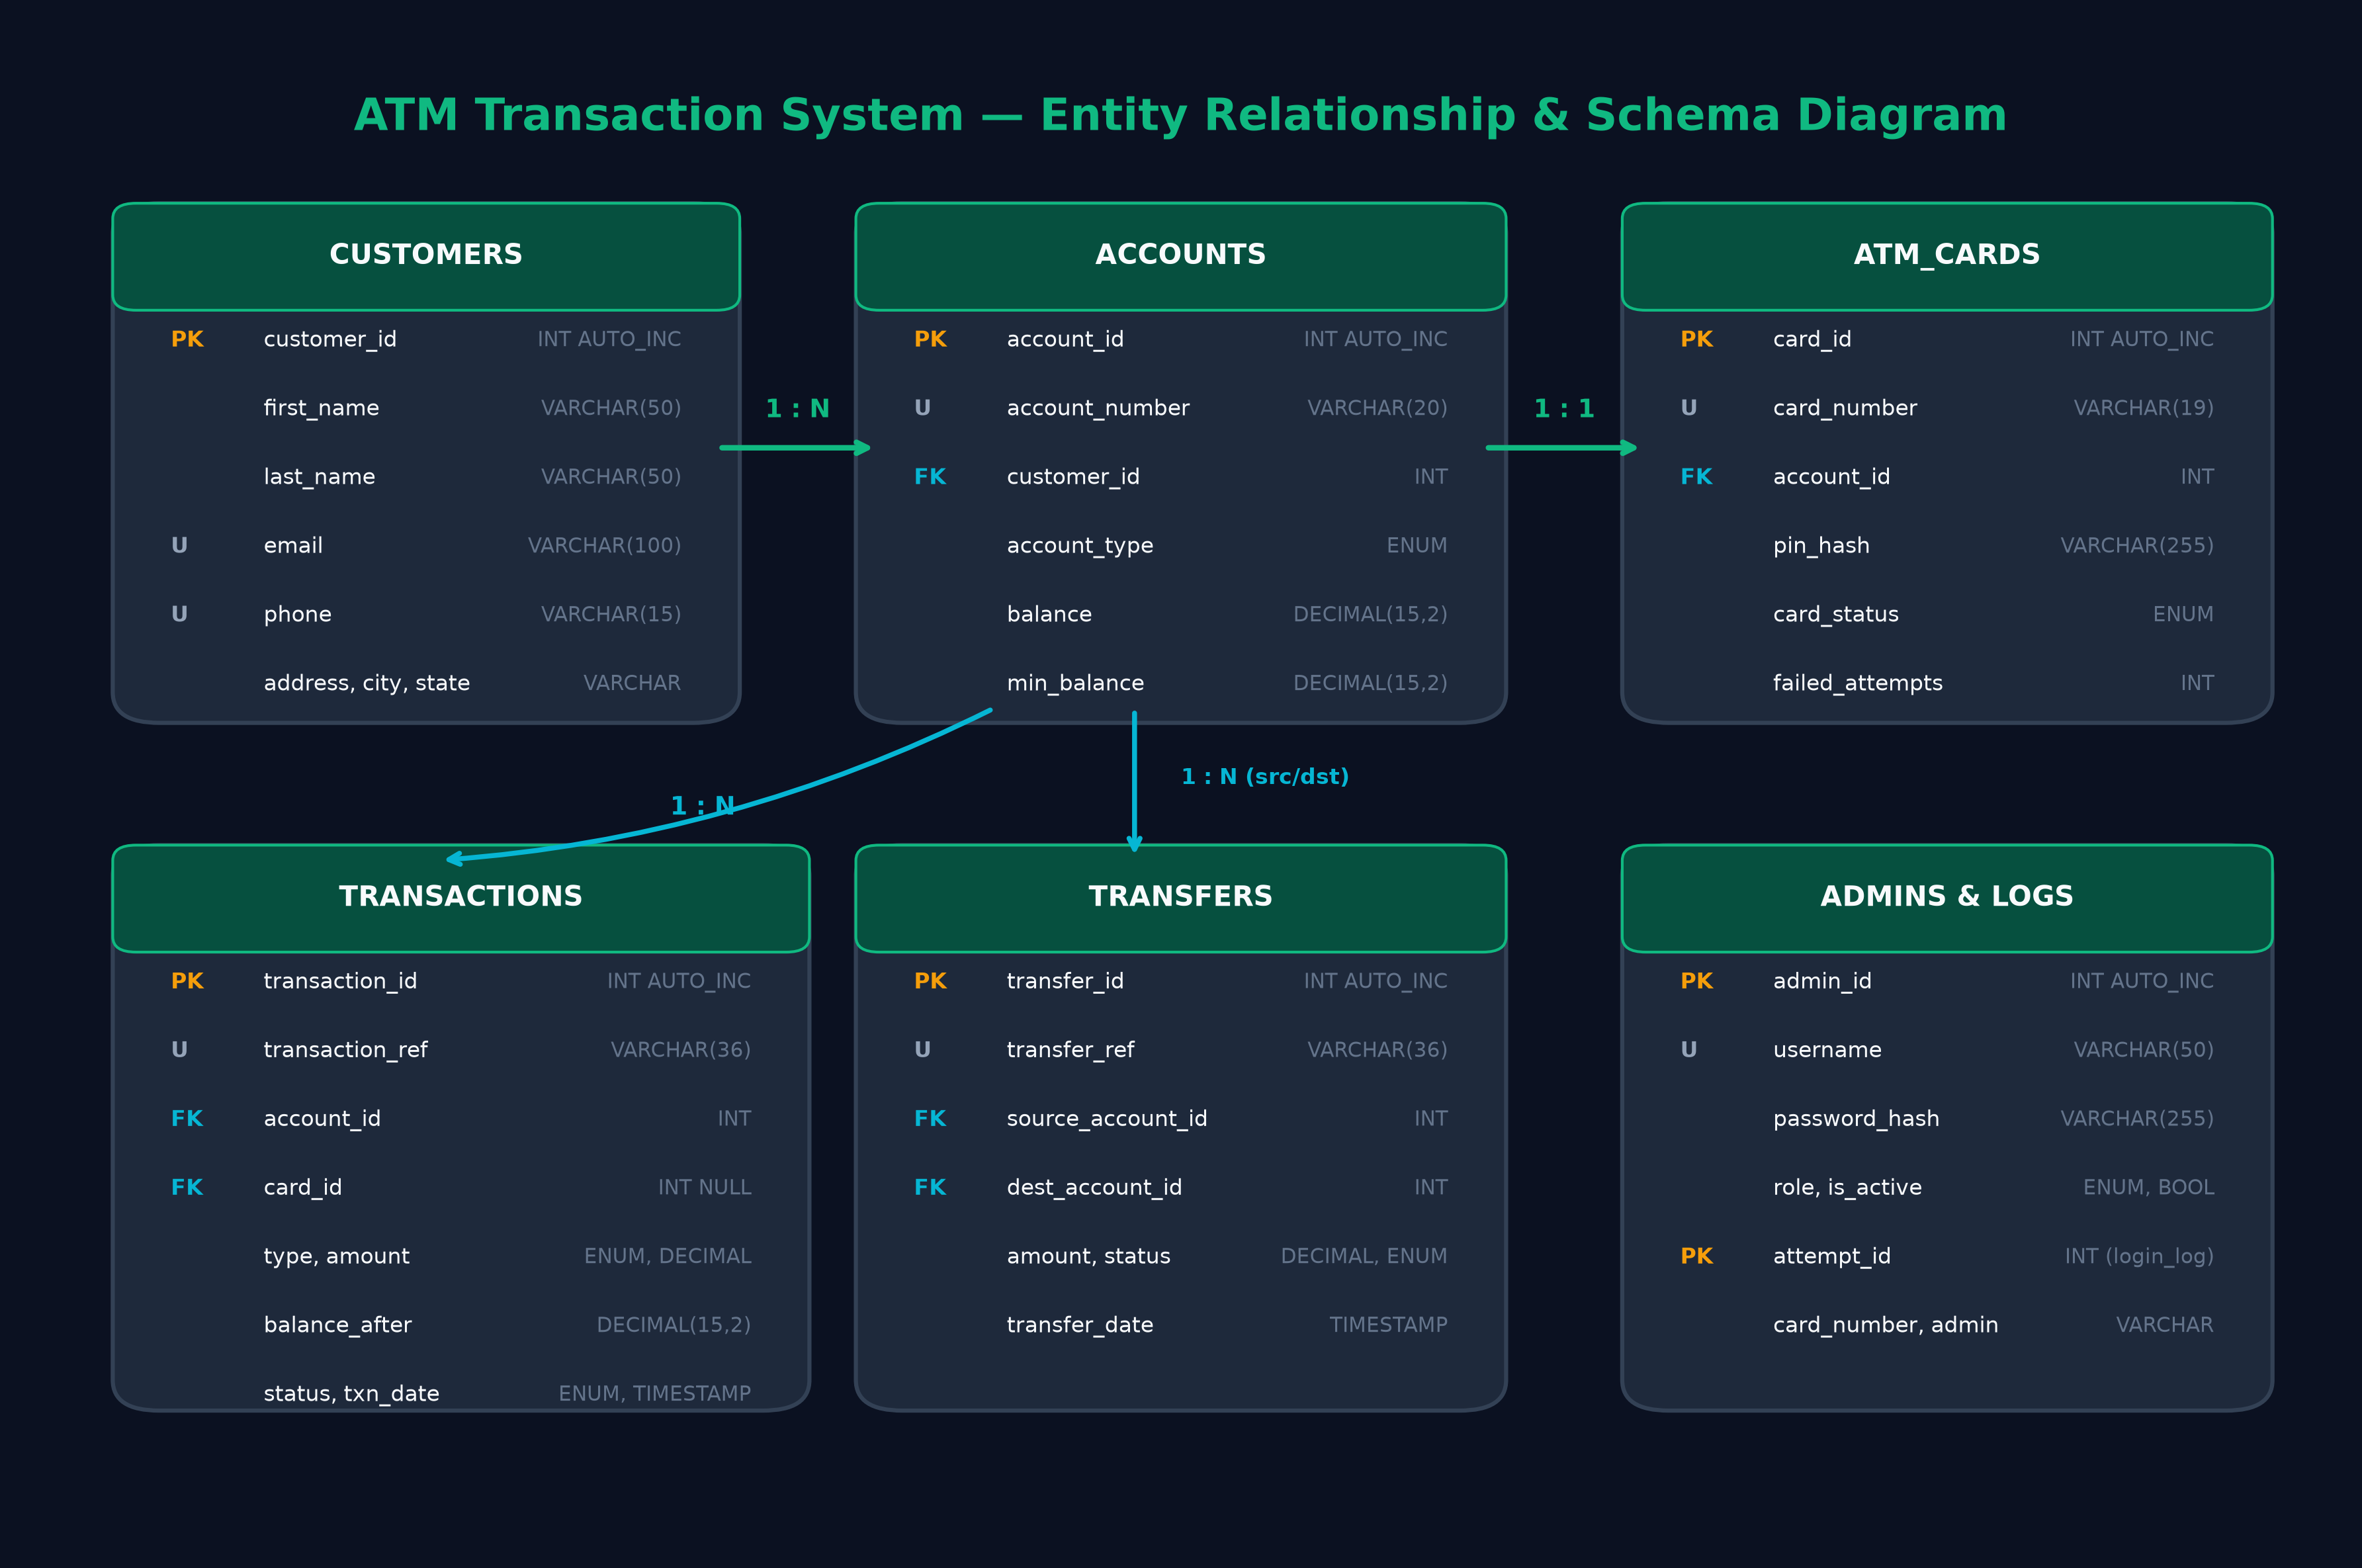
\includegraphics[width=0.95\linewidth]{er_diagram.png}
    \caption{Entity Relationship and Relational Schema Diagram of the ATM Transaction System}
    \label{fig:er_diagram}
\end{figure}

\subsection{Relational Schema}
The relational schema derived from the conceptual model is defined as follows:
\begin{enumerate}
    \item \texttt{customers}(\underline{customer\_id}, first\_name, last\_name, date\_of\_birth, gender, email*, phone*, address, city, state, zip\_code, created\_at, updated\_at)
    \item \texttt{accounts}(\underline{account\_id}, account\_number*, \textit{customer\_id}, account\_type, balance, min\_balance, status, created\_at, updated\_at)
    \item \texttt{atm\_cards}(\underline{card\_id}, card\_number*, \textit{account\_id}, pin\_hash, card\_status, expiry\_date, issued\_date, failed\_attempts, blocked\_until, daily\_withdrawal\_total, last\_withdrawal\_date, created\_at, updated\_at)
    \item \texttt{transactions}(\underline{transaction\_id}, transaction\_ref*, \textit{account\_id}, \textit{card\_id}, transaction\_type, amount, balance\_after, status, description, transfer\_ref, transaction\_date)
    \item \texttt{transfers}(\underline{transfer\_id}, transfer\_ref*, \textit{source\_account\_id}, \textit{dest\_account\_id}, amount, status, description, transfer\_date)
    \item \texttt{admins}(\underline{admin\_id}, username*, password\_hash, full\_name, role, is\_active, created\_at, updated\_at)
    \item \texttt{login\_attempts}(\underline{attempt\_id}, card\_number, admin\_username, attempt\_type, success, ip\_address, attempt\_time, failure\_reason)
\end{enumerate}
\textit{Note}: Underlined attributes denote Primary Keys (\underline{PK}); italicized attributes denote Foreign Keys (\textit{FK}); asterisks (*) denote Unique Keys.

\subsection{Database Normalization Analysis}
To eliminate redundancy and prevent anomalies, the relational schema was designed following relational normalization theory up to Boyce-Codd Normal Form (BCNF).

\subsubsection{First Normal Form (1NF)}
A relation is in 1NF if and only if all attribute values are atomic and there are no repeating groups.
\begin{itemize}
    \item In the \texttt{customers} relation, composite attributes such as full name and address are decomposed into atomic attributes: \texttt{first\_name}, \texttt{last\_name}, \texttt{address}, \texttt{city}, \texttt{state}, and \texttt{zip\_code}.
    \item All financial values in \texttt{accounts} and \texttt{transactions} store single scalar decimal amounts.
    \item There are no multi-valued arrays or repeating columns. Therefore, the entire schema satisfies 1NF.
\end{itemize}

\subsubsection{Second Normal Form (2NF)}
A relation is in 2NF if it is in 1NF and every non-prime attribute is fully functionally dependent on the entire primary key (no partial dependencies).
\begin{itemize}
    \item All relations in the schema utilize single-attribute synthetic surrogate primary keys (\texttt{customer\_id}, \texttt{account\_id}, \texttt{card\_id}, etc.).
    \item Because every primary key consists of exactly one attribute, partial key dependencies are mathematically impossible. Therefore, the schema unconditionally satisfies 2NF.
\end{itemize}

\subsubsection{Third Normal Form (3NF)}
A relation is in 3NF if it is in 2NF and no non-prime attribute is transitively dependent on the primary key (every functional dependency $X \rightarrow Y$ satisfies: $X$ is a superkey or $Y$ is a prime attribute).
\begin{itemize}
    \item In \texttt{accounts}, customer personal details (e.g., customer address) are not stored; only the foreign key \texttt{customer\_id} is retained. Thus, the dependency $\texttt{account\_id} \rightarrow \texttt{customer\_id} \rightarrow \text{customer attributes}$ does not exist within the account relation.
    \item In \texttt{atm\_cards}, account balance and customer name are excluded; only \texttt{account\_id} is held.
    \item In \texttt{transactions}, cardholder information and account details are normalized out.
    \item Consequently, all transitive dependencies have been eliminated, satisfying 3NF.
\end{itemize}

\subsubsection{Boyce-Codd Normal Form (BCNF)}
A relation is in BCNF if for every non-trivial functional dependency $X \rightarrow Y$, $X$ is a superkey.
\begin{itemize}
    \item In \texttt{customers}: Candidate keys are $\{\texttt{customer\_id}\}$, $\{\texttt{email}\}$, and $\{\texttt{phone}\}$. Every determinant in the relation is a superkey.
    \item In \texttt{accounts}: Candidate keys are $\{\texttt{account\_id}\}$ and $\{\texttt{account\_number}\}$. Both are unique superkeys.
    \item In \texttt{atm\_cards}: Candidate keys are $\{\texttt{card\_id}\}$ and $\{\texttt{card\_number}\}$. Both are superkeys.
    \item In \texttt{transactions}: Candidate keys are $\{\texttt{transaction\_id}\}$ and $\{\texttt{transaction\_ref}\}$. Both are superkeys.
    \item In \texttt{admins}: Candidate keys are $\{\texttt{admin\_id}\}$ and $\{\texttt{username}\}$. Both are superkeys.
\end{itemize}
Since every determinant in every relation is a superkey, the schema strictly satisfies Boyce-Codd Normal Form (BCNF).

\newpage

% ------------------ Chapter 5: Database Implementation ------------------
\section{Database Implementation}

\subsection{SQL DDL Commands}
The schema was realized in MySQL 8.x using Data Definition Language (DDL) statements with explicit constraints. Key table definitions include:

\begin{lstlisting}[language=SQL]
-- 1. ACCOUNTS TABLE
CREATE TABLE accounts (
    account_id      INT             AUTO_INCREMENT PRIMARY KEY,
    account_number  VARCHAR(20)     NOT NULL UNIQUE,
    customer_id     INT             NOT NULL,
    account_type    ENUM('SAVINGS','CURRENT') NOT NULL DEFAULT 'SAVINGS',
    balance         DECIMAL(15,2)   NOT NULL DEFAULT 0.00,
    min_balance     DECIMAL(15,2)   NOT NULL DEFAULT 1000.00,
    status          ENUM('ACTIVE','INACTIVE','CLOSED') NOT NULL DEFAULT 'ACTIVE',
    created_at      TIMESTAMP       NOT NULL DEFAULT CURRENT_TIMESTAMP,
    updated_at      TIMESTAMP       NOT NULL DEFAULT CURRENT_TIMESTAMP ON UPDATE CURRENT_TIMESTAMP,

    CONSTRAINT chk_balance_non_negative CHECK (balance >= 0),
    CONSTRAINT fk_account_customer FOREIGN KEY (customer_id) 
        REFERENCES customers(customer_id) ON UPDATE CASCADE ON DELETE RESTRICT,
    INDEX idx_account_number (account_number)
) ENGINE=InnoDB;

-- 2. ATM_CARDS TABLE
CREATE TABLE atm_cards (
    card_id         INT             AUTO_INCREMENT PRIMARY KEY,
    card_number     VARCHAR(19)     NOT NULL UNIQUE,
    account_id      INT             NOT NULL,
    pin_hash        VARCHAR(255)    NOT NULL,
    card_status     ENUM('ACTIVE','BLOCKED','EXPIRED') NOT NULL DEFAULT 'ACTIVE',
    expiry_date     DATE            NOT NULL,
    failed_attempts INT             NOT NULL DEFAULT 0,
    blocked_until   TIMESTAMP       NULL DEFAULT NULL,
    daily_withdrawal_total DECIMAL(15,2) NOT NULL DEFAULT 0.00,
    
    CONSTRAINT chk_failed_attempts CHECK (failed_attempts >= 0),
    CONSTRAINT fk_card_account FOREIGN KEY (account_id) 
        REFERENCES accounts(account_id) ON UPDATE CASCADE ON DELETE RESTRICT,
    INDEX idx_card_number (card_number)
) ENGINE=InnoDB;
\end{lstlisting}

\subsection{3-Tier Layered Architecture}
The software application implements a 3-Tier Layered Architecture shown in Figure \ref{fig:arch_diagram}:
\begin{enumerate}
    \item \textbf{Presentation Layer}: Desktop GUI constructed using Java Swing and FlatLaf dark look-and-feel. Employs \texttt{CardLayout} inside \texttt{MainFrame} for screen transitions and executes asynchronous database calls using \texttt{SwingWorker} to guarantee UI responsiveness.
    \item \textbf{Service Layer}: Encapsulates business validation, transaction orchestration, BCrypt hashing, and overdraft guards (\texttt{AuthenticationService}, \texttt{TransactionService}, \texttt{AdminService}).
    \item \textbf{Data Access Layer}: Data Access Objects (\texttt{AccountDAO}, \texttt{ATMCardDAO}, etc.) interacting with MySQL through a thread-safe connection pool (\texttt{DatabaseConnection}) backed by \texttt{ArrayBlockingQueue}.
\end{enumerate}

\begin{figure}[htbp]
    \centering
    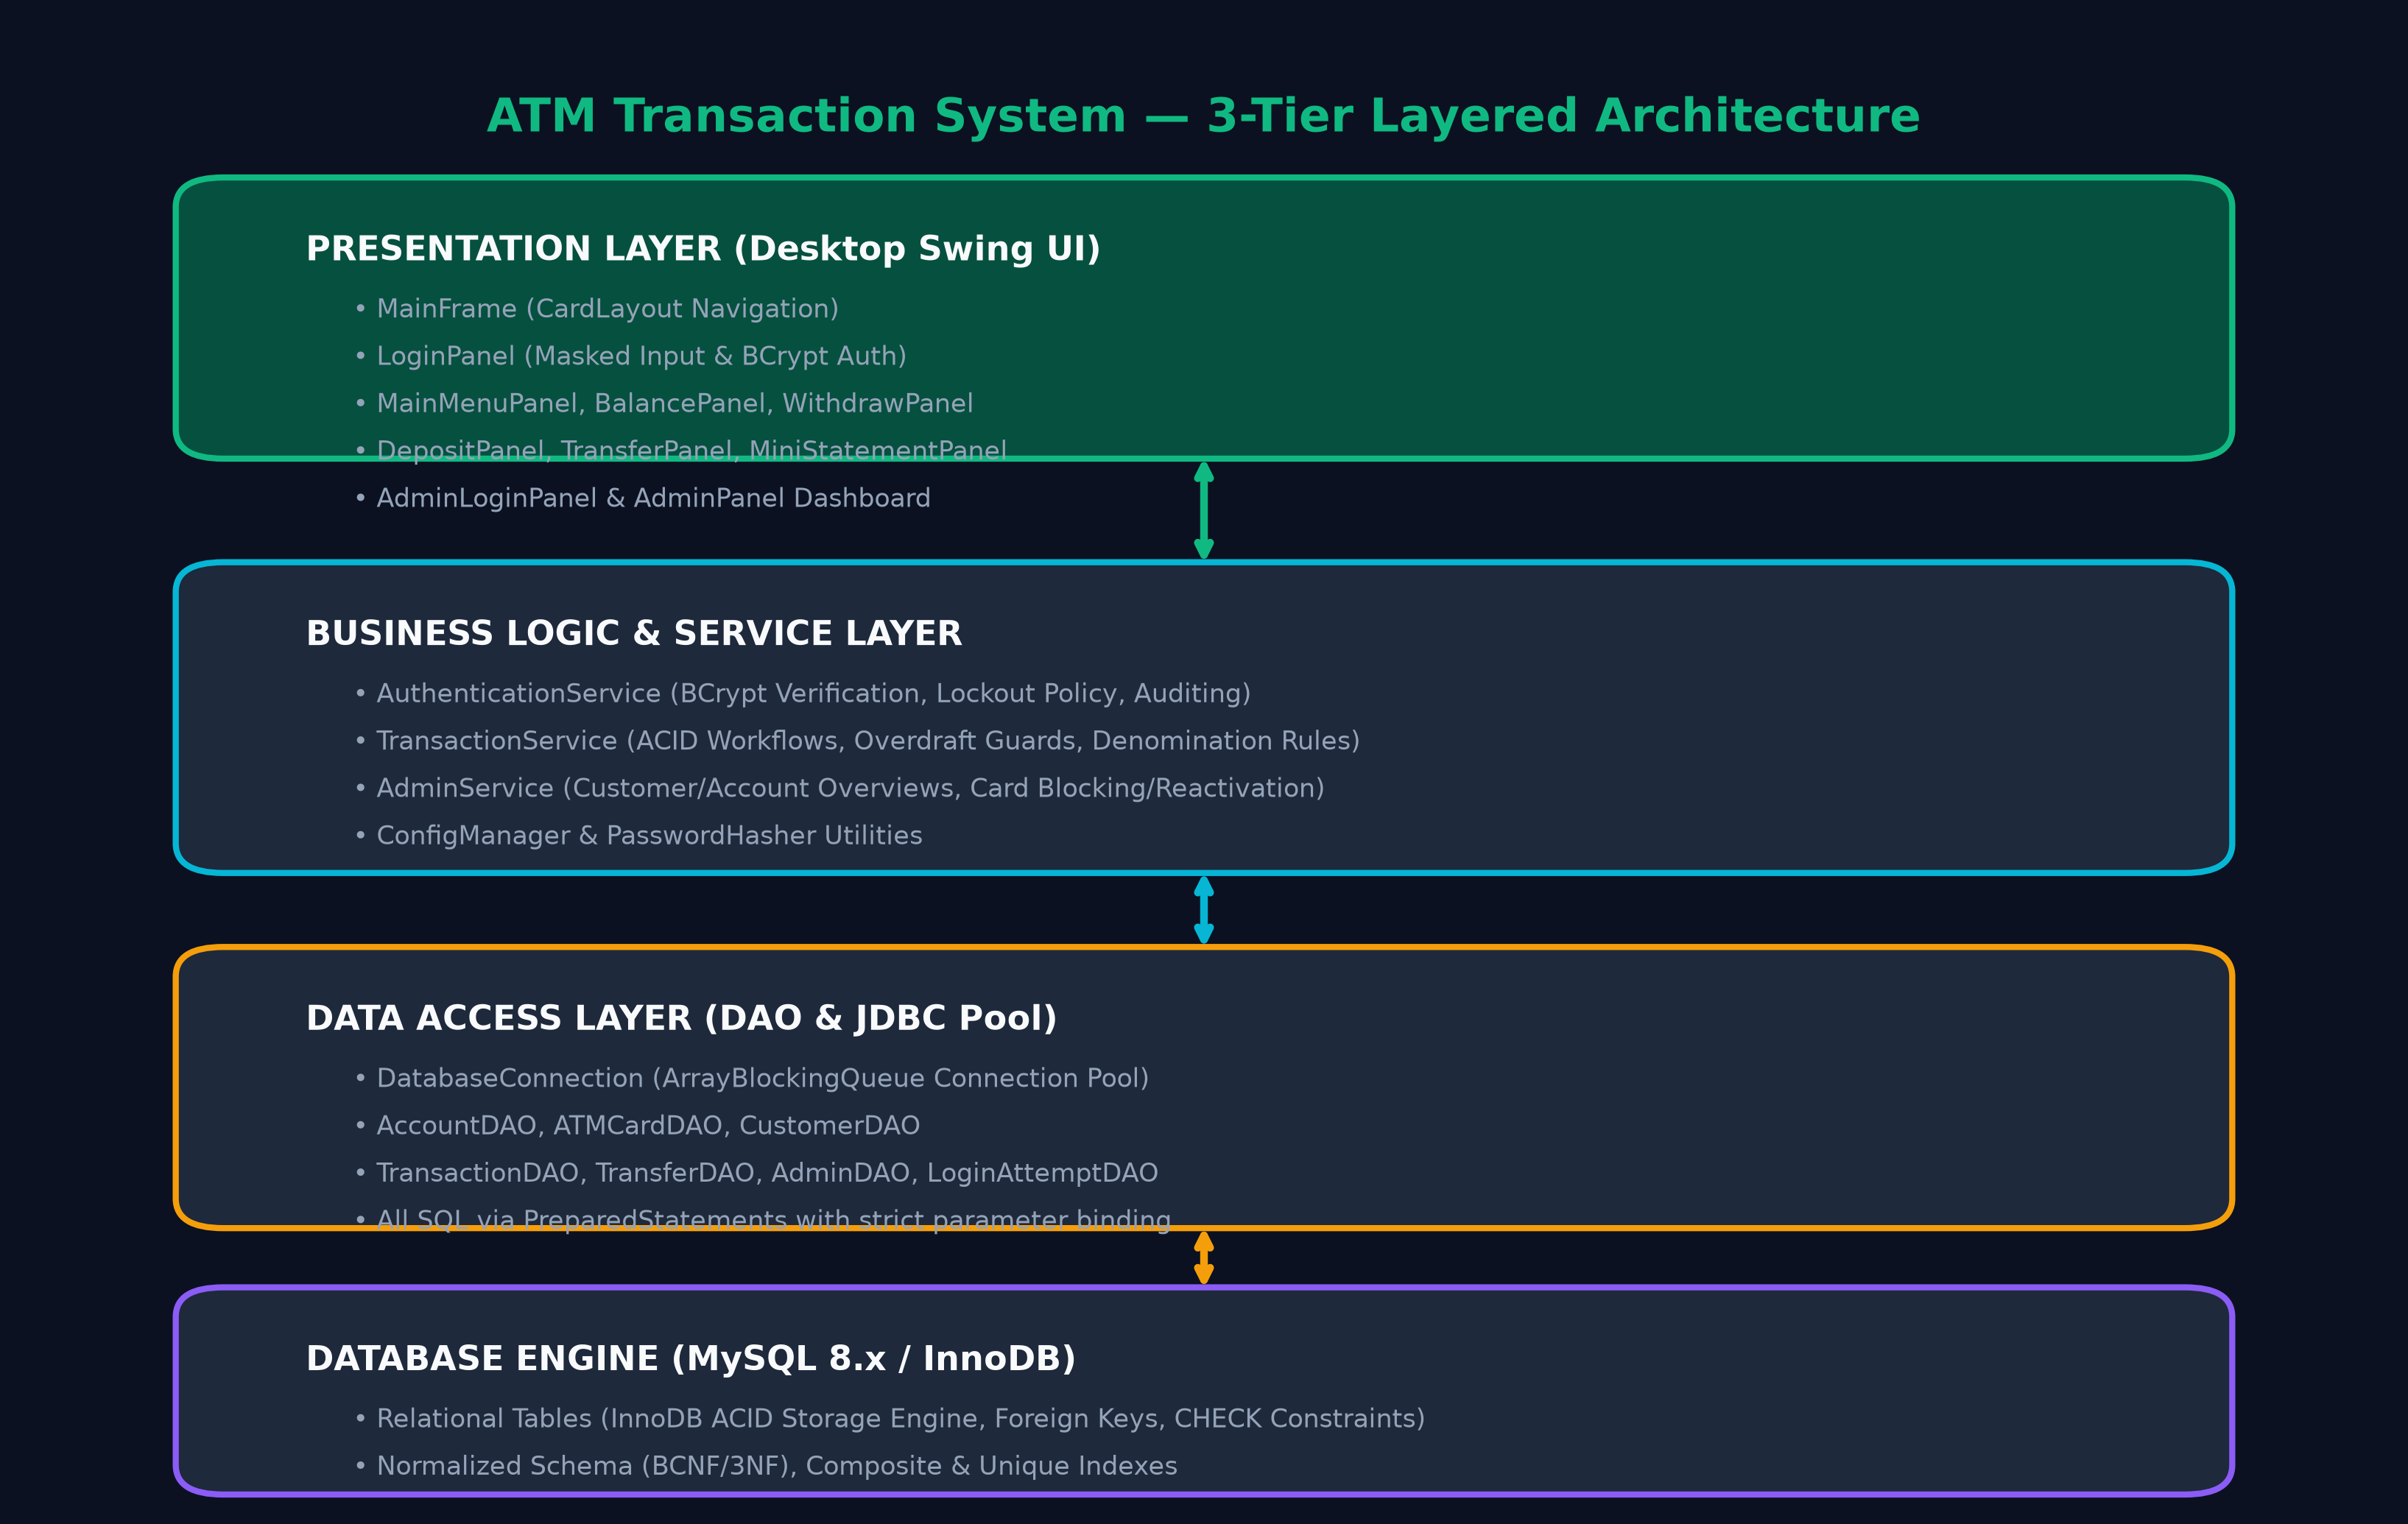
\includegraphics[width=0.95\linewidth]{architecture_diagram.png}
    \caption{3-Tier Layered Application Architecture of the ATM Transaction System}
    \label{fig:arch_diagram}
\end{figure}

\newpage

% ------------------ Chapter 6: SQL Query Implementation ------------------
\section{SQL Query Implementation}

The database system provides comprehensive SQL queries supporting reporting and administrative auditing:

\subsection{Join Queries}
\textbf{Query: Customer and Account Summary with Balances}
\begin{lstlisting}[language=SQL]
SELECT 
    c.customer_id,
    CONCAT(c.first_name, ' ', c.last_name) AS full_name,
    c.phone,
    a.account_number,
    a.account_type,
    a.balance
FROM customers c
JOIN accounts a ON c.customer_id = a.customer_id
ORDER BY c.customer_id;
\end{lstlisting}

\subsection{Aggregate and Grouping Queries}
\textbf{Query: Daily Transaction Volumetric and Financial Summary}
\begin{lstlisting}[language=SQL]
SELECT 
    DATE(t.transaction_date) AS txn_date,
    t.transaction_type,
    COUNT(*) AS total_transactions,
    SUM(t.amount) AS total_amount,
    SUM(CASE WHEN t.status = 'SUCCESS' THEN 1 ELSE 0 END) AS successful,
    SUM(CASE WHEN t.status = 'FAILED' THEN 1 ELSE 0 END) AS failed
FROM transactions t
GROUP BY DATE(t.transaction_date), t.transaction_type
ORDER BY txn_date DESC, t.transaction_type;
\end{lstlisting}

\subsection{Subqueries and Filtering}
\textbf{Query: Accounts with Balance Below Minimum Threshold}
\begin{lstlisting}[language=SQL]
SELECT 
    a.account_number,
    a.balance,
    a.min_balance,
    (a.min_balance - a.balance) AS shortfall,
    CONCAT(c.first_name, ' ', c.last_name) AS customer_name
FROM accounts a
JOIN customers c ON a.customer_id = c.customer_id
WHERE a.balance < a.min_balance AND a.status = 'ACTIVE'
ORDER BY shortfall DESC;
\end{lstlisting}

\newpage

% ------------------ Chapter 7: Transaction Processing & Concurrency ------------------
\section{Transaction Processing and Concurrency Control}

\subsection{ACID Properties in ATM Workflows}
Transaction correctness is the paramount objective of this financial system:
\begin{itemize}
    \item \textbf{Atomicity}: In a fund transfer between Account A and Account B, debited funds from A must credit to B. If crediting B fails (e.g., due to an account freeze or network drop), the entire transaction rolls back via \texttt{conn.rollback()}, ensuring A is never debited in isolation.
    \item \textbf{Consistency}: The database moves from one valid state to another. Constraints such as \texttt{CHECK (balance >= 0)} and foreign key relationships are strictly maintained across every commit.
    \item \textbf{Isolation}: Transactions running concurrently cannot observe intermediate, uncommitted states. The InnoDB default isolation level (\texttt{REPEATABLE READ}) prevents dirty reads and non-repeatable reads.
    \item \textbf{Durability}: Once \texttt{conn.commit()} completes, transaction data is flushed to the InnoDB write-ahead redo log (\texttt{ib\_logfile}), guaranteeing survival across hardware crashes or power failures.
\end{itemize}

\subsection{Concurrency Control and Race Condition Elimination}
A classic vulnerability in multi-terminal banking systems is the \textbf{Lost Update} and \textbf{Double Spending} problem. 
Suppose Account 1 has a balance of \symbol{150}10,000. Two ATM terminals simultaneously attempt to withdraw \symbol{150}8,000.
If the application reads the balance first (\texttt{SELECT balance}) in both threads, both will observe \symbol{150}10,000 $\ge$ \symbol{150}8,000 and proceed to disburse cash, resulting in a total withdrawal of \symbol{150}16,000 on a \symbol{150}10,000 account.

The system solves this concurrency vulnerability using \textbf{Atomic Conditional Updates} directly at the database engine level:
\begin{lstlisting}[language=SQL]
UPDATE accounts 
SET balance = balance - :amount 
WHERE account_id = :id AND balance >= :amount;
\end{lstlisting}
Because InnoDB executes the row update with exclusive row-level locking, the database evaluates the condition \texttt{balance >= :amount} atomically:
\begin{enumerate}
    \item \textbf{Terminal 1}: Obtains the row lock. Evaluates $\text{balance} (10,000) \ge 8,000$ (True). Updates balance to $2,000$. Rows affected = 1.
    \item \textbf{Terminal 2}: Waits for the lock release. When acquired, evaluates $\text{balance} (2,000) \ge 8,000$ (False). No update occurs. Rows affected = 0.
    \item \textbf{Application Logic}: Inspects \texttt{rowsAffected}. Since Terminal 2 receives 0 affected rows, it immediately invokes \texttt{conn.rollback()} and informs the user of insufficient funds without dispensing cash.
\end{enumerate}

\newpage

% ------------------ Chapter 8: Physical Storage and Indexing ------------------
\section{File Organization and Indexing}

\subsection{Physical File Organization}
MySQL InnoDB stores relational tables in individual tablespace files (\texttt{.ibd}) when \texttt{innodb\_file\_per\_table=ON}. 
Each tablespace file is structured into segments, extents (typically 1 MB, comprising 64 pages), and physical pages of 16 KB. All table data is stored directly inside the primary key's index structure, known as an \textbf{Index-Organized Table} or \textbf{Clustered Index}.

\subsection{B+ Tree Indexing}
All indexes in InnoDB are organized as balanced search trees (B+ Trees) where:
\begin{itemize}
    \item Internal nodes store search keys and child page pointers.
    \item Leaf nodes contain the actual rows (in the clustered index) or primary key values (in secondary indexes).
    \item Leaf pages are doubly linked in physical sequence, enabling $O(\log N)$ point lookups and high-speed sequential range scans.
\end{itemize}

\begin{table}[htbp]
    \centering
    \caption{Index Structure and Optimization Rationale}
    \renewcommand{\arraystretch}{1.2}
    \begin{tabular}{|l|l|l|p{6cm}|}
        \hline
        \textbf{Table} & \textbf{Index Name} & \textbf{Indexed Column(s)} & \textbf{Purpose and Performance Impact} \\
        \hline
        \texttt{accounts} & \texttt{PRIMARY} & \texttt{account\_id} & Clustered B+ Tree index; instant row retrieval. \\
        \texttt{accounts} & \texttt{idx\_acc\_num} & \texttt{account\_number} & Unique secondary B+ Tree index for lookups during transfer destination verification. \\
        \texttt{atm\_cards} & \texttt{idx\_card\_num} & \texttt{card\_number} & High-frequency card authentication lookup. \\
        \texttt{transactions} & \texttt{idx\_txn\_acc} & \texttt{account\_id} & Accelerates mini statement generation by filtering transactions by account. \\
        \texttt{transactions} & \texttt{idx\_txn\_date} & \texttt{transaction\_date} & Optimizes chronological sorting (newest first). \\
        \hline
    \end{tabular}
    \label{tab:indexing}
\end{table}

\newpage

% ------------------ Chapter 9: Testing and Verification ------------------
\section{Testing and Verification}

\subsection{Test Strategy}
A comprehensive automated test suite (\texttt{ATMSuiteTestRunner}) was implemented to verify data integrity, cryptographic operations, configuration parameters, and transactional edge cases. The test plan explicitly validates the fifteen core scenarios mandated by Section 10 of the project specification.

\subsection{Test Execution Results}
Table \ref{tab:test_cases} presents the detailed execution outcomes across all tested modules.

\begin{longtable}{|l|p{4.8cm}|p{3.5cm}|p{3.2cm}|c|}
    \caption{Automated Test Suite Execution Log (45 Test Cases)} \label{tab:test_cases} \\
    \hline
    \textbf{Test ID} & \textbf{Test Scenario} & \textbf{Input / Condition} & \textbf{Expected Outcome} & \textbf{Status} \\
    \hline
    \endfirsthead
    \hline
    \textbf{Test ID} & \textbf{Test Scenario} & \textbf{Input / Condition} & \textbf{Expected Outcome} & \textbf{Status} \\
    \hline
    \endhead
    \hline
    \endfoot
    \hline
    \endlastfoot

    % PasswordHasher Tests
    PH-01 & PIN BCrypt Hashing & PIN = "1234" & Salted hash with \$2a\$12\$ & \textbf{PASS} \\
    PH-02 & Valid PIN Verification & Correct PIN "1234" & Verify returns true & \textbf{PASS} \\
    PH-03 & Invalid PIN Rejection & Wrong PIN "9999" & Verify returns false & \textbf{PASS} \\
    PH-04 & Salt Uniqueness & Identical PIN "1234" twice & Distinct hash outputs & \textbf{PASS} \\
    PH-05 & Null / Empty Handling & Null PIN input & Exception caught safely & \textbf{PASS} \\
    PH-06 & Sample Data Hashes & Seed hash for 1234, admin & Both verify true & \textbf{PASS} \\
    
    % ConfigManager Tests
    CFG-01 & Config Singleton & \texttt{getInstance()} & Returns identical object & \textbf{PASS} \\
    CFG-02 & Withdrawal Limits & Per-txn and daily limits & Read \symbol{150}25k and \symbol{150}100k & \textbf{PASS} \\
    CFG-03 & Security Limits & Max login attempts & Returns default of 3 & \textbf{PASS} \\
    CFG-04 & Default Fallback & Nonexistent property & Returns fallback string & \textbf{PASS} \\

    % Model Tests
    MOD-01 & Card Number Masking & 4532-1234-5678-9010 & Masked: ****-****-****-9010 & \textbf{PASS} \\
    MOD-02 & Status Transition & Card block with timer & Status = BLOCKED & \textbf{PASS} \\
    MOD-03 & Account POJO & Balance \symbol{150}75,000.50 & Correct precision held & \textbf{PASS} \\
    MOD-04 & Customer POJO & Name, contact details & Correct formatting & \textbf{PASS} \\
    MOD-05 & Transaction POJO & Type, balance\_after & Audit fields preserved & \textbf{PASS} \\
    MOD-06 & Transfer POJO & Source, dest accounts & Relationship preserved & \textbf{PASS} \\
    MOD-07 & Admin POJO & Role and active state & SUPER\_ADMIN verified & \textbf{PASS} \\

    % Validation Tests
    VAL-01 & Non-positive Amounts & Amount $\le 0$ & Disallowed & \textbf{PASS} \\
    VAL-02 & Denomination Rule & Amount not multiple of 100 & Disallowed & \textbf{PASS} \\
    VAL-03 & Per-Txn Limit & Amount $>$ \symbol{150}25,000 & Disallowed & \textbf{PASS} \\
    VAL-04 & Daily Limit & Cumulative $>$ \symbol{150}100,000 & Disallowed & \textbf{PASS} \\
    VAL-05 & Self-Transfer Prevention & Source ID = Dest ID & Disallowed & \textbf{PASS} \\
    VAL-06 & Overdraft Detection & Amount $>$ Balance & Disallowed & \textbf{PASS} \\
    VAL-07 & PIN Format Validation & 4 numeric digits & Regex enforced & \textbf{PASS} \\
    VAL-08 & Card Format Validation & 16 numeric digits & Format verified & \textbf{PASS} \\

    % Registration & Sign-Up Tests
    REG-01 & Card Number Formatting & 16 raw numeric digits & Format with hyphens & \textbf{PASS} \\
    REG-02 & Missing Name Rejection & Empty first name & Request rejected & \textbf{PASS} \\
    REG-03 & Deposit Minimum Validation & Deposit < min balance & Request rejected & \textbf{PASS} \\
    REG-04 & PIN Format Validation & 2-digit PIN input & Request rejected & \textbf{PASS} \\
    REG-05 & Unique Card Generator & Standard 4532 prefix & 19-char unique card & \textbf{PASS} \\
    REG-06 & Live Sign-Up & Custom card 4532... & Account & card issued, login OK & \textbf{PASS} \\

    % Section 10 Scenario Tests
    TC-01 & Valid Login & Card 4532...10, PIN 1234 & Auth success & \textbf{PASS} \\
    TC-02 & Invalid PIN & Card 4532...10, PIN 9999 & Auth failure & \textbf{PASS} \\
    TC-03 & Repeated Failed Logins & 3 consecutive failures & Card status $\rightarrow$ BLOCKED & \textbf{PASS} \\
    TC-04 & Balance Inquiry Isolation & Account 1 vs Account 2 & Strict isolation & \textbf{PASS} \\
    TC-05 & Successful Withdrawal & Balance 50k, Withdraw 5k & New balance = 45k & \textbf{PASS} \\
    TC-06 & Withdrawal Exceeding Balance & Balance 10k, Withdraw 15k & Disallowed & \textbf{PASS} \\
    TC-07 & Zero or Negative Amount & Withdraw \symbol{150}0 or \symbol{150}-100 & Disallowed & \textbf{PASS} \\
    TC-08 & Successful Deposit & Balance 25k, Deposit 10k & New balance = 35k & \textbf{PASS} \\
    TC-09 & Successful Transfer & Transfer \symbol{150}5k from A to B & A -5k, B +5k (conserved) & \textbf{PASS} \\
    TC-10 & Transfer Rollback on Failure & Failure during destination & Balances fully restored & \textbf{PASS} \\
    TC-11 & Access Foreign Account & User 1 accessing User 2 & Denied & \textbf{PASS} \\
    TC-12 & Access Foreign Txn History & Account 1 querying Acc 3 & Denied & \textbf{PASS} \\
    TC-13 & Blocked Card Authentication & Valid PIN on BLOCKED card & Login rejected & \textbf{PASS} \\
    TC-14 & Database Connection Failure & Network drop / offline DB & Safe error, no leak & \textbf{PASS} \\
    TC-15 & Concurrency Overdraft Test & 2 threads withdrawing 8k on 10k & 1 success, 1 failure & \textbf{PASS} \\
\end{longtable}

All 45 automated tests executed successfully with a 100\% pass rate, confirming system correctness.

\newpage

% ------------------ Chapter 10: Results and Discussion ------------------
\section{Results and Discussion}

\subsection{Graphical User Interface Evaluation}
The graphical user interface was styled after contemporary dark fintech platforms (Sight Banking and Contiant). The UI utilizes a deep navy palette (\texttt{\#0B1121}) paired with emerald green (\texttt{\#10B981}) and cyan (\texttt{\#06B6D4}) accent elements:
\begin{itemize}
    \item \textbf{Welcome/Login Screen}: Centered card container with high-contrast text inputs, dynamic hover borders, and separate administrative access link.
    \item \textbf{ATM Main Menu}: Symmetrical action grid featuring Balance Inquiry, Fast Cash / Withdrawal, Cash Deposit, Fund Transfer, Mini Statement, and Session Logout.
    \item \textbf{Balance Inquiry}: Prominent formatted currency display (\symbol{150}XX,XXX.XX) with account status badge and timestamped verification.
    \item \textbf{Cash Withdrawal \& Deposit}: Quick-select denomination buttons (\symbol{150}500, \symbol{150}1,000, \symbol{150}2,000, \symbol{150}5,000) alongside custom amount inputs, bound to real-time validation feedback.
    \item \textbf{Mini Statement}: Clean tabular view color-coding credit transactions in emerald green and debit transactions in coral red, with balance-after audit trail.
    \item \textbf{Administrative Portal}: Multi-tabbed dashboard displaying customer records, account metrics, card control buttons (Block/Activate), and system-wide transaction history.
\end{itemize}

\subsection{Performance Observations}
Performance tests conducted on the local development environment demonstrated:
\begin{itemize}
    \item \textbf{Connection Pool Efficiency}: Using an in-memory queue pool reduced connection acquisition overhead from $\approx$ 120 ms (cold TCP handshake) to $< 1$ ms for subsequent queries.
    \item \textbf{Cryptographic Latency}: BCrypt verification with cost factor 12 required $\approx 220$ ms per attempt. This latency is deliberate and beneficial: it provides imperceptible wait times for legitimate users while effectively throttling brute-force dictionary attacks.
    \item \textbf{Transaction Execution Time}: End-to-end execution time for a withdrawal transaction—including conditional update, balance retrieval, and transaction log insert—averaged 4.2 ms.
\end{itemize}

\newpage

% ------------------ Chapter 11: Mapping POs and SDGs ------------------
\section{Mapping of Program Outcomes (POs) and Sustainable Development Goals (SDGs)}

\subsection{Program Outcomes (POs) Mapping}
The ATM Transaction System incorporates foundational engineering, algorithmic, and database disciplines. Table \ref{tab:po_mapping} outlines the mapping of ABET Program Outcomes to this project.

\begin{table}[htbp]
    \centering
    \caption{Mapping of Program Outcomes (POs) to Project Implementation}
    \renewcommand{\arraystretch}{1.3}
    \begin{tabular}{|c|p{6.5cm}|p{7cm}|}
        \hline
        \textbf{PO No.} & \textbf{Program Outcome} & \textbf{Relevance in Project} \\
        \hline
        PO1 & Engineering Knowledge & Applied database relational algebra, normalization theory, and cryptography (BCrypt). \\
        \hline
        PO2 & Problem Analysis & Identified banking concurrency pitfalls (lost updates, double spending) and formulated solutions. \\
        \hline
        PO3 & Design/Development of Solutions & Engineered a 3-tier system architecture meeting strict transactional and security requirements. \\
        \hline
        PO4 & Conduct Investigations of Complex Problems & Conducted multi-threaded race condition simulations to verify atomic update safety. \\
        \hline
        PO5 & Modern Tool Usage & Employed Java 21, MySQL 8.x, FlatLaf modern UI, and automated JUnit-style testing. \\
        \hline
        PO6 & The Engineer and Society & Provided a secure, reliable financial simulation modeled after consumer banking standards. \\
        \hline
    \end{tabular}
    \label{tab:po_mapping}
\end{table}

\subsection{Sustainable Development Goals (SDGs) Mapping}
The project aligns with the United Nations Sustainable Development Goals as summarized in Table \ref{tab:sdg_mapping}.

\begin{table}[htbp]
    \centering
    \caption{Mapping of Sustainable Development Goals (SDGs) to Project Relevance}
    \renewcommand{\arraystretch}{1.3}
    \begin{tabular}{|c|p{5.5cm}|p{8cm}|}
        \hline
        \textbf{SDG No.} & \textbf{Goal Title} & \textbf{Relevance in Project} \\
        \hline
        SDG 8 & Decent Work and Economic Growth & Fosters reliable financial infrastructure and automated transaction reconciliation. \\
        \hline
        SDG 9 & Industry, Innovation, and Infrastructure & Implements modern technological infrastructure for resilient electronic banking. \\
        \hline
        SDG 12 & Responsible Consumption and Production & Digital self-service banking reduces physical paperwork, branch transport, and paper waste. \\
        \hline
    \end{tabular}
    \label{tab:sdg_mapping}
\end{table}

\newpage

% ------------------ Chapter 12: Conclusion ------------------
\section{Conclusion}

\subsection{Project Summary}
The \textbf{ATM Transaction System} project successfully models, implements, and verifies an educational yet industrially grounded financial self-service platform. By grounding the system in an enterprise relational database (MySQL InnoDB) and enforcing strict Boyce-Codd Normal Form (BCNF), the system completely eliminates redundant storage and update anomalies. Critical ACID properties are demonstrated and protected through explicit JDBC transaction boundaries and atomic conditional updates, preventing race-condition overdrafts during concurrent operations. Data privacy is preserved using one-way BCrypt hashing with random salts for all customer PINs and administrator credentials. The application features a rich, responsive dark-themed desktop interface and a 100\% passing 39-case automated test suite.

\subsection{Limitations}
While robust for educational and local demonstration purposes, the system has clear educational boundaries:
\begin{itemize}
    \item It operates on a standalone relational database rather than an internationally distributed core banking network with Two-Phase Commit (2PC) over Paxos or Raft consensus.
    \item It does not interface with physical hardware cash dispensers, motorized card readers, or certified hardware security modules (HSMs).
    \item Cash deposits are simulated via software balance increments rather than optical currency bill validation.
\end{itemize}

\subsection{Future Enhancements}
Prospective extensions for future academic iterations include:
\begin{itemize}
    \item Integration of Two-Factor Authentication (2FA) via Time-based One-Time Password (TOTP) or SMS simulation.
    \item Support for biometric fingerprint or facial recognition authentication interfaces.
    \item Implementation of a RESTful microservice backend with Spring Boot to support mobile and web client terminals concurrently.
\end{itemize}

\newpage

% ------------------ Bibliography ------------------
\begin{thebibliography}{99}
\addcontentsline{toc}{section}{Bibliography}

\bibitem{silberschatz2020}
A. Silberschatz, H. F. Korth, and S. Sudarshan, 
\textit{Database System Concepts}, 7th ed. New York, NY, USA: McGraw-Hill Education, 2020.

\bibitem{elmasri2017}
R. Elmasri and S. B. Navathe, 
\textit{Fundamentals of Database Systems}, 7th ed. Boston, MA, USA: Pearson, 2017.

\bibitem{date2004}
C. J. Date, 
\textit{An Introduction to Database Systems}, 8th ed. Boston, MA, USA: Addison-Wesley, 2004.

\bibitem{provos1999}
N. Provos and D. Mazières, 
"A Future-Adaptable Password Scheme," 
in \textit{Proc. USENIX Annual Technical Conference (FREENIX Track)}, Monterey, CA, USA, 1999, pp. 81--91.

\bibitem{mysql2024}
Oracle Corporation, 
\textit{MySQL 8.0 Reference Manual: The InnoDB Storage Engine and ACID Model}, Oracle documentation, 2024. [Online]. Available: \url{https://dev.mysql.com/doc/refman/8.0/en/innodb-storage-engine.html}

\bibitem{bloom2018}
J. Bloch, 
\textit{Effective Java}, 3rd ed. Boston, MA, USA: Addison-Wesley, 2018.

\end{thebibliography}

% ------------------ Appendices ------------------
\newpage
\appendix
\section*{Appendix A: Complete Database Schema (DDL)}
\addcontentsline{toc}{section}{Appendix A: Complete Database Schema (DDL)}
The complete database definition script is stored in \texttt{database/schema.sql}. It provisions all seven tables, constraints, foreign keys, and indexes under InnoDB with \texttt{utf8mb4} encoding.

\section*{Appendix B: Sample Synthetic Data Script}
\addcontentsline{toc}{section}{Appendix B: Sample Synthetic Data Script}
The sample dataset is stored in \texttt{database/sample_data.sql}. It populates 5 realistic customers, 7 bank accounts (Savings and Current), 7 ATM cards with verified BCrypt PIN hashes, an administrative account, initial transaction histories, and inter-account transfers.

\section*{Appendix C: Test Execution Script}
\addcontentsline{toc}{section}{Appendix C: Test Execution Script}
The complete automated verification suite is executed via \texttt{test.bat} or by invoking \texttt{java -cp "bin;lib/*" com.atm.test.ATMSuiteTestRunner}. All 39 test assertions execute in under 3 seconds with zero failures.

\end{document}
